\section{Números}

\questao{A diretora Sheyla tem uma calculadora diferente das demais. Sua calculadora não possui teclas de operações e em seu lugar tem-se teclas com as letras E, M, S e P. Cada tecla possui uma habilidade:}
E - Pega o número colocado na tela e multiplica por 6 e subtrai dois 
\begin{figure}[htbp]
  \centering
  % Coluna da esquerda: Imagem
  \begin{minipage}{0.3\textwidth}
    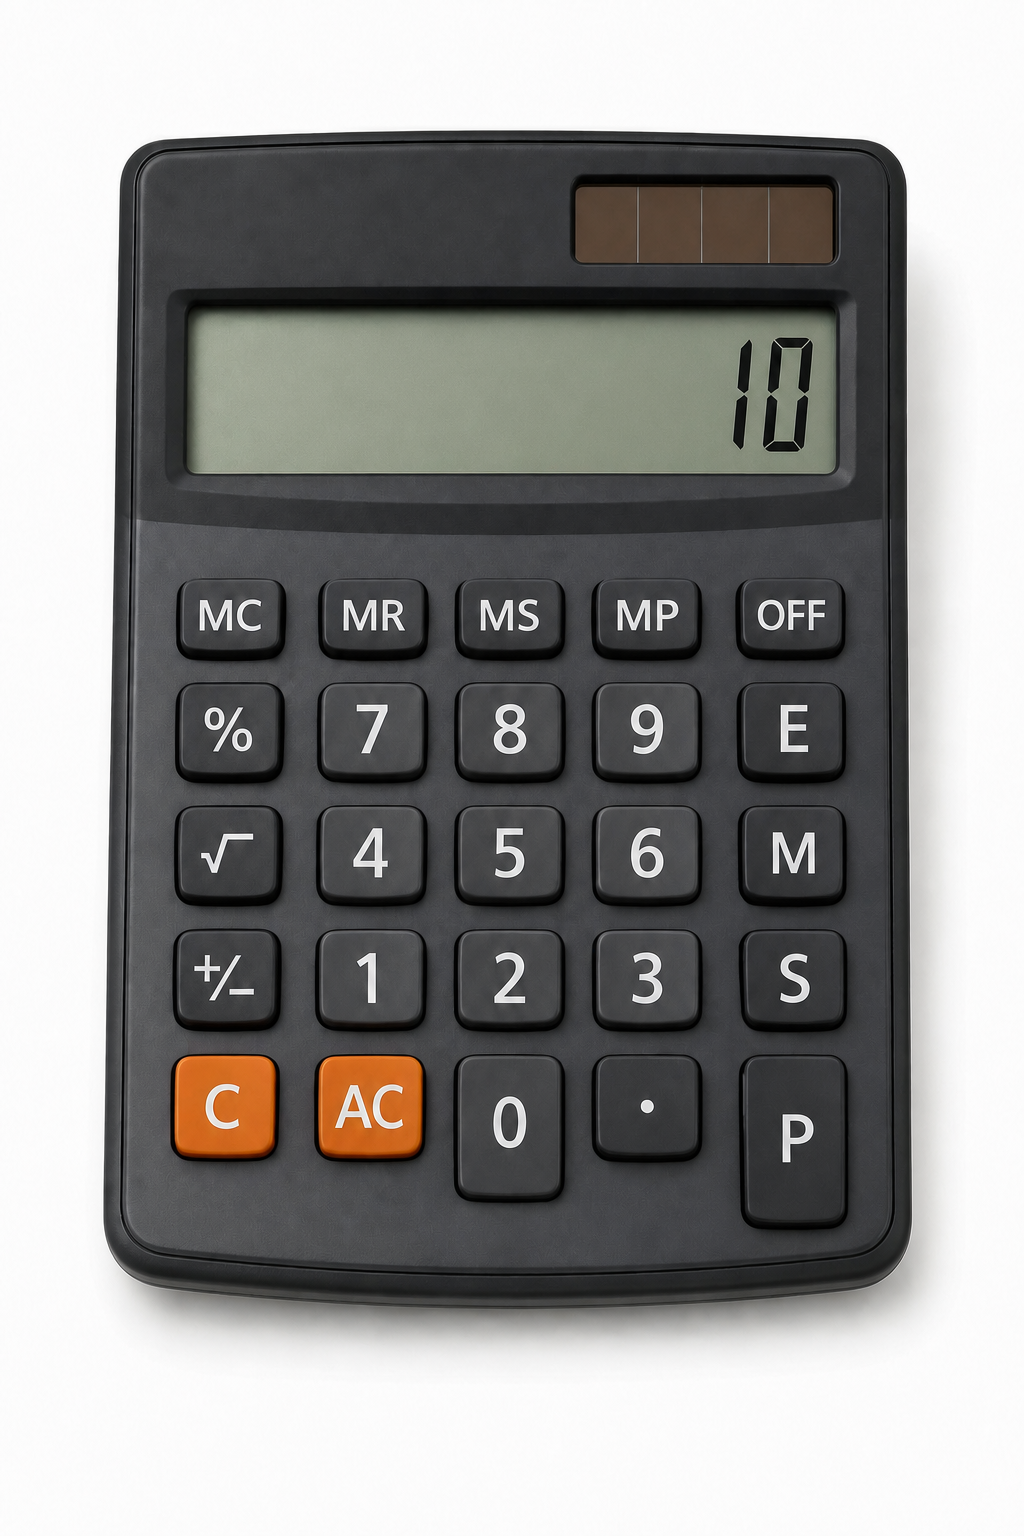
\includegraphics[width=\textwidth]{figuras/6_ano/IMG_0914.png} % Substitua pelo nome do seu arquivo
    \label{fig:minha_foto}
  \end{minipage}
  \hfill % Preenche o espaço entre as duas colunas
  % Coluna da direita: Texto
  \begin{minipage}{0.6\textwidth}
    \begin{itemize}
            \item  A tecla $E$ faz com que o número que está na tela seja multiplicado por 6 e após isso o resultado é subtraído por dois.
            \item  A tecla $M$ faz com que o número que está na tela seja dividido por dois e após isso o resultado é subtraído por cinco
            \item A tecla $S$ faz com que o número que está na tela permaneça o mesmo.
            \item A tecla $P$ faz com que o número que está na tela se transforme em zero.
        \end{itemize}
  \end{minipage}
\end{figure}
\begin{enumerate}[label=\alph*)]
    \item Na tela da calculadora da diretora Sheyla tem-se o número 10, igual a imagem da calculador. Se ela apertar em seguidas as teclas $E-M-P$, qual será o resultado apresentado na tela?
   
    \item Na tela da calculadora da diretora Sheyla tem-se o número 10, igual a imagem da calculador. Se ela apertar em seguidas as teclas $E-E-S-P-S-P$, qual será o resultado apresentado na tela?
    
    \item Na tela da calculadora da diretora Sheyla tem-se o número 10, igual a imagem da calculador. Se ela apertar em seguidas as teclas $E-E-E-S-M-S-E$, qual será o resultado apresentado na tela?
\end{enumerate}

\begin{solucoes}{1}
    \solucao
    \textbf{item a)}

    Para resolvermos o item a) é preciso observarmos apenas o último comando. Se observarmos a pergunta, a última tecla apresentada é a tecla $P$ que tem como função transformar o número da tela em 0. Logo, independentemente do que fizermos antes, o resultado final será 0. 

    \solucao
    \textbf{item b)}
    
       Para resolvermos o item b) é preciso observarmos apenas o último comando. Se observarmos a pergunta, a última tecla apresentada é a tecla $P$ que tem como função transformar o número da tela em 0. Logo, independentemente do que fizermos antes, o resultado final será 0 (Perceba que a quantidade de operações foi maior apenas para ver o nível de leitura, interpretação e estratégia de quem tentar resolvê-la).

\solucao
\textbf{item c)}

No item c) é preciso que se faça a série de execuções que se pedem. Na tela temos o número 10 e assim, fazendo $E-E-E-S-M-S-E$
\begin{equation*}
    10\cdot 6=60-2=58
\end{equation*}
\begin{equation*}
    58\cdot6=348-2=346
\end{equation*}
\begin{equation*}
    346\cdot 6=2076-2=2074 
\end{equation*}
Como a letra $S$ repete o mesmo resultado vamos ao próximo passo
\begin{equation*}
    \frac{2074}{2}=1037-5=1032
\end{equation*}
Por fim, 
\begin{equation*}
    1032\cdot6=6192-2=6190             
\end{equation*}
Portanto, o resultado na tela será $6190$.
       
\end{solucoes}

\questao{(OAM 2025 - Nível 1) A professora Joyce escreveu no quadro todos os divisores positivos do número $2025$.
Sabendo que ela levou exatamente $3$ segundos para escrever cada divisor, quanto tempo, em segundos,
ela gastou para escrever apenas os divisores de $2025$ que são múltiplos de $3$?}

\begin{solucoes}{1}
    \solucao
    Ao fatorar o número $2025$,tem-se, \\
    
    \begin{tabular}{r|l}
        $2025$ & $5$ \\
         $405$ & $5$ \\
         $81$ & $3$ \\
         $27$ & $3$ \\ 
         $9$ & $3$ \\
         $3$ & $3$\\ \cline{2-2}
         $1$ & $5^2\cdot 3^4$
    \end{tabular}
\\\\
Logos, podemos determinar a quantidade de divisores do número $2025$,onde $(2+1)\cdot (4+1)=3\cdot5=15$. São $15$ divisores, onde temos,

\begin{equation*}
    D_{2025}= \left\{ 1,3,5,9,15,25,27,45,75,81,135,225,405,675,2025\right\}
\end{equation*}

Os números $ \left\{3,9,15,27,45,75,81,135, 225, 405,675,2025\right\}$ são divisores de $2025$ e múltiplos de $3$ e como ela levou $3s$ para escrever cada um, temos $12\cdot 3=36s$.     
\end{solucoes}

\questao{(OAM 2025 - Nível 1) Um número é adoisado quando ele pode ser obtido pela soma de duas potências de $2$.
Por exemplo, $12$ é adoisado porque $12 =2^3 + 2^2$. Quantos números adoisados menores do que 1000
existem?}

\begin{solucoes}{2}
\solucao
Podemos separar em dois casos, potências iguais e potências diferentes. 

$i)$ Se as potências forem iguais, temos $9$ possibilidades, pois. $2^9+2^9=1024$ que é maior que $1000$.

$ii)$ Se as potências forem diferentes, temos $10$ possibilidades para a primeira escolha e $9$ para a segunda, logo $10\cdot 9=90$. Todavia, $2^8+2^9=2^9+2^8$ e assim precisamos dividir por dois para não contarmos duas vezes $\frac{90}{2}=45$.

Sendo assim, o total de números adoisados é $9+45=54$.
    
    \solucao
Sabemos que um número é adoisado quando ele pode ser obtido pela soma de duas potências de $2$ e queremos determinar a quantidade de números adoisados menores que $1000$. Até 1000 temos as potências $2^0=1$, $2^1=2$, $2^2=4$, $2^3=8$, $2^4=16$, $2^5=32$, $2^6=64$, $2^7=128$, $2^8=256$ e $2^9=512$, pois $2^{10}=1024$ que passa de $1000$. Logo, temos 10 números para serem somados. Vamos fixar um e variar os outros e descobriremos todos os casos,
\\\\
$1)$ Fixemos o $2^0=1$ e temos $10$ números que são adoisados. 
\\\\
$2)$ Fixemos o $2^1=2$ e tiremos os números $3=2^0+2^1$ que já foi computado no primeiro caso e assim temos $9$ números adoisados. 
\\\\
$3)$ Fixemos  o $2^2=4$ e tiremos os números $5=2^0+2^2$ e $6=2^1+2^2$ que já foram computados nos casos anteriores e assim temos $8$ números adoisados.
\\\\
$4)$ Fixemos  o $2^3=8$ e tiremos os números $9=2^0+2^3$, $10=2^1+2^3$ e $12=2^2+2^3$ que já foram computados nos casos anteriores e assim temos $7$ números adoisados.
\\\\
$5)$ Fixemos  o $2^4=16$ e tiremos os números $17=2^0+2^4$, $18=2^1+2^4$, $20=2^2+2^4$ e $24=2^3+2^4$ que já foram computados nos casos anteriores e assim temos $6$ números adoisados.
\\\\
$6)$ Fixemos  o $2^5=32$ e tiremos os números $33=2^0+2^5$, $34=2^1+2^5$, $36=2^2+2^5$, $40=2^3+2^5$ e $48=2^4+2^5$ que já foram computados nos casos anteriores e assim temos $5$ números adoisados.
\\\\
$7)$ Fixemos  o $2^6=64$ e tiremos os números $65=2^0+2^6$, $66=2^1+2^6$, $68=2^2+2^6$, $72=2^3+2^6$, $80=2^4+2^6$ e $96=2^5+2^6$ que já foram computados nos casos anteriores e assim temos $4$ números adoisados.
\\\\
$8)$ Fixemos  o $2^7=128$ e tiremos os números $129=2^0+2^7$, $130=2^1+2^7$, $132=2^2+2^7$, $136=2^3+2^7$, $144=2^4+2^7$, $160=2^5+2^7$ e $192=2^6+2^7$ que já foram computados nos casos anteriores e assim temos $3$ números adoisados.
\\\\
$9)$Fixemos  o $2^8=256$ e tiremos os números $257=2^0+2^8$, $258=2^1+2^8$, $260=2^2+2^8$, $264=2^3+2^8$, $272=2^4+2^8$, $288=2^5+2^8$, $320=2^6+2^8$ e $384=2^7+2^8$ que já foram computados nos casos anteriores e assim temos $2$ números adoisados.
\\\\ 
$10)$ Por fim, não há nenhum número novo, pois a única possibilidade nova é $1024=2^9+2^9$.
\\\\

Logo, temos um total de $10+9+8+7+6+5+4+3+2=54$ números adoisados.

\end{solucoes}






